\documentclass[11pt]{article}

\usepackage[margin=1in]{geometry}
\usepackage{amsmath,amssymb}
\usepackage{booktabs}
\usepackage{array}
\usepackage{caption}
\usepackage{subcaption}
\usepackage{graphicx}
\usepackage{hyperref}
\usepackage{url}
\usepackage{enumitem}
\usepackage{xcolor}
\usepackage{longtable}
\usepackage{multirow}
\usepackage{microtype}
\usepackage[numbers,sort&compress]{natbib}

\hypersetup{
  colorlinks=true,
  linkcolor=blue!50!black,
  citecolor=blue!50!black,
  urlcolor=blue!50!black
}

\newcommand{\method}{GCPM}
\newcommand{\vect}[1]{\mathbf{#1}}
\newcommand{\score}{\mathrm{score}}
\newcommand{\simfn}{\mathrm{sim}}

\title{\textbf{Graph-Guided Compressed Procedural Memory for Web Agents}\\
\large A Research-Internship Study on Mind2Web and WebArena}

\author{Ammar\\
Research Internship Project}

\date{\today}

\begin{document}
\maketitle

\begin{abstract}
Large-language-model web agents often solve each task from scratch, even when prior interactions contain reusable procedural knowledge. This paper studies a graph-guided procedural memory architecture for web agents that abstracts prior trajectories into reusable policies, retrieves relevant memories for new tasks, and guards against negative transfer from failed procedures. The method combines compact workflow representations, relation-aware retrieval, negative memory, and context-conscious prompting in order to improve reuse while controlling memory and retrieval overhead. The system is evaluated in both offline and live web-agent settings. The results indicate that procedural memory can improve task-level behavior while making the memory layer more efficient and interpretable. More broadly, the study argues that web-agent memory should be treated as a joint learning, retrieval, and systems problem rather than as prompt augmentation alone.
\end{abstract}

\section{Introduction}

Web agents are expected to transform natural-language goals into long-horizon browser interactions. A task such as finding a product attribute, checking an order status, filtering search results, or extracting review evidence often requires many state-dependent actions. Modern LLM agents can perform such tasks with reasoning-and-acting loops \citep{yao2023react}, but repeated web tasks contain substantial procedural reuse. A shopping review-extraction task and another shopping review-extraction task differ in entities and page ids, yet share the same high-level routine: navigate to product reviews, scan or paginate, verify textual evidence, and answer in the required format.

Agent Workflow Memory (AWM) \citep{wang2024awm} captures this intuition by inducing workflows from successful trajectories and retrieving them for future tasks. The present project extends that idea into a more explicit systems architecture. Instead of treating workflow memory as only prompt text, the implementation separates: (i) durable structured memories, (ii) compact searchable text, (iii) vector embeddings, (iv) graph relations between procedures and task families, (v) negative memories derived from failures, (vi) retrieval-event logging, and (vii) compressed ANN backends. This design is evaluated in two settings:

\begin{itemize}[leftmargin=*]
  \item \textbf{Mind2Web} \citep{deng2023mind2web}, using recorded exemplar trajectories for local offline evaluation and retrieval benchmarking.
  \item \textbf{WebArena} \citep{zhou2023webarena}, using a live EC2-hosted WebArena stack with BrowserGym/Playwright execution and a shopping-domain procedural memory.
\end{itemize}

The contribution is not a new benchmark, but an implementation study of how procedural memory should be engineered for speed, storage, and reuse. The project asks three questions:

\begin{enumerate}[leftmargin=*]
  \item Can AWM-style procedural reuse be implemented end-to-end for Mind2Web and WebArena with paper-style metrics and reproducible evaluation methodology?
  \item Which memory optimizations materially reduce retrieval latency and storage footprint?
  \item What additional architecture is required for live WebArena execution, where browser state, page loading, answer formatting, and negative transfer matter?
\end{enumerate}

\section{Related Work}

\paragraph{Workflow memory for agents.}
AWM \citep{wang2024awm} induces reusable workflows from web-agent trajectories and retrieves them in offline and online settings. The work reports improvements on Mind2Web and WebArena, motivating this project. The implementation here follows the broad procedural-memory motivation but changes the storage and retrieval layer: workflows are stored as structured, graph-linked, compressed, and queryable memories rather than only as prompt snippets.

\paragraph{Web-agent benchmarks.}
Mind2Web \citep{deng2023mind2web} provides over 2,000 web tasks across 137 websites and 31 domains, with annotated action sequences on real websites. WebArena \citep{zhou2023webarena} provides a reproducible suite of live websites, including e-commerce, forums, GitLab-like development, Wikipedia-like content, map tools, and external knowledge. BrowserGym \citep{dechezelles2024browsergym} standardizes web-agent environments and provides a gym-like interface for observations and actions.

\paragraph{Approximate nearest-neighbor retrieval.}
The memory layer is a retrieval system over workflow embeddings. FAISS \citep{johnson2017faiss} provides efficient exact and approximate similarity search, including compressed-domain search. HNSW \citep{malkov2020hnsw} uses navigable small-world graphs for approximate nearest-neighbor search. Product quantization (PQ) \citep{jegou2011pq}, optimized product quantization (OPQ) \citep{ge2013opq}, and anisotropic vector quantization \citep{guo2019avq} reduce vector memory and accelerate search. DiskANN \citep{subramanya2019diskann} is relevant for future billion-scale disk-resident procedural memory. Recent quantizers such as RaBitQ \citep{gao2024rabitq} and TurboQuant \citep{zandieh2025turboquant} are relevant to low-bit vector compression and online quantization.

\paragraph{Sentence embeddings.}
The implementation uses sentence-transformer-style dense embeddings. Sentence-BERT \citep{reimers2019sentencebert} established efficient sentence embeddings for similarity search. BGE-style embeddings \citep{chen2024bge} are used in the WebArena retrieval benchmark because they provide strong compact dense representations for retrieval.

\section{Problem Formulation}

Let a web task be specified by a natural-language goal $g$, a website or domain $d$, and a sequence of browser observations and actions. A trajectory is:
\begin{equation}
  \tau = \left(g, d, \{(o_t, a_t, r_t)\}_{t=1}^{T}\right),
\end{equation}
where $o_t$ is the DOM/accessibility observation at step $t$, $a_t$ is the executed action, and $r_t$ is reward or correctness feedback when available. A procedural memory item is an abstraction:
\begin{equation}
  p_i = \mathcal{A}(\tau_i),
\end{equation}
where $\mathcal{A}$ maps a concrete trajectory to reusable procedural guidance. The abstraction should preserve the task family, action skeleton, evidence requirements, answer format, and stopping condition, while discarding brittle element ids and page-specific clutter.

At test time, a new state $x_t=(g,o_t,d,h_t)$ is converted into a memory query $q_t$, where $h_t$ is action history. The memory system retrieves a set $R_t$:
\begin{equation}
  R_t = \operatorname*{TopK}_{p_i \in \mathcal{M}} \score(q_t,p_i),
\end{equation}
subject to an acceptance gate. If no memory passes the threshold, the LLM solves from the current page state without procedural advice.

\section{System Overview}

Figure~\ref{fig:flowchart} shows the implemented architecture. The system has four major loops: online interaction, memory-augmented decision making, long-term procedural memory, and post-task learning.

\begin{figure}[t]
  \centering
  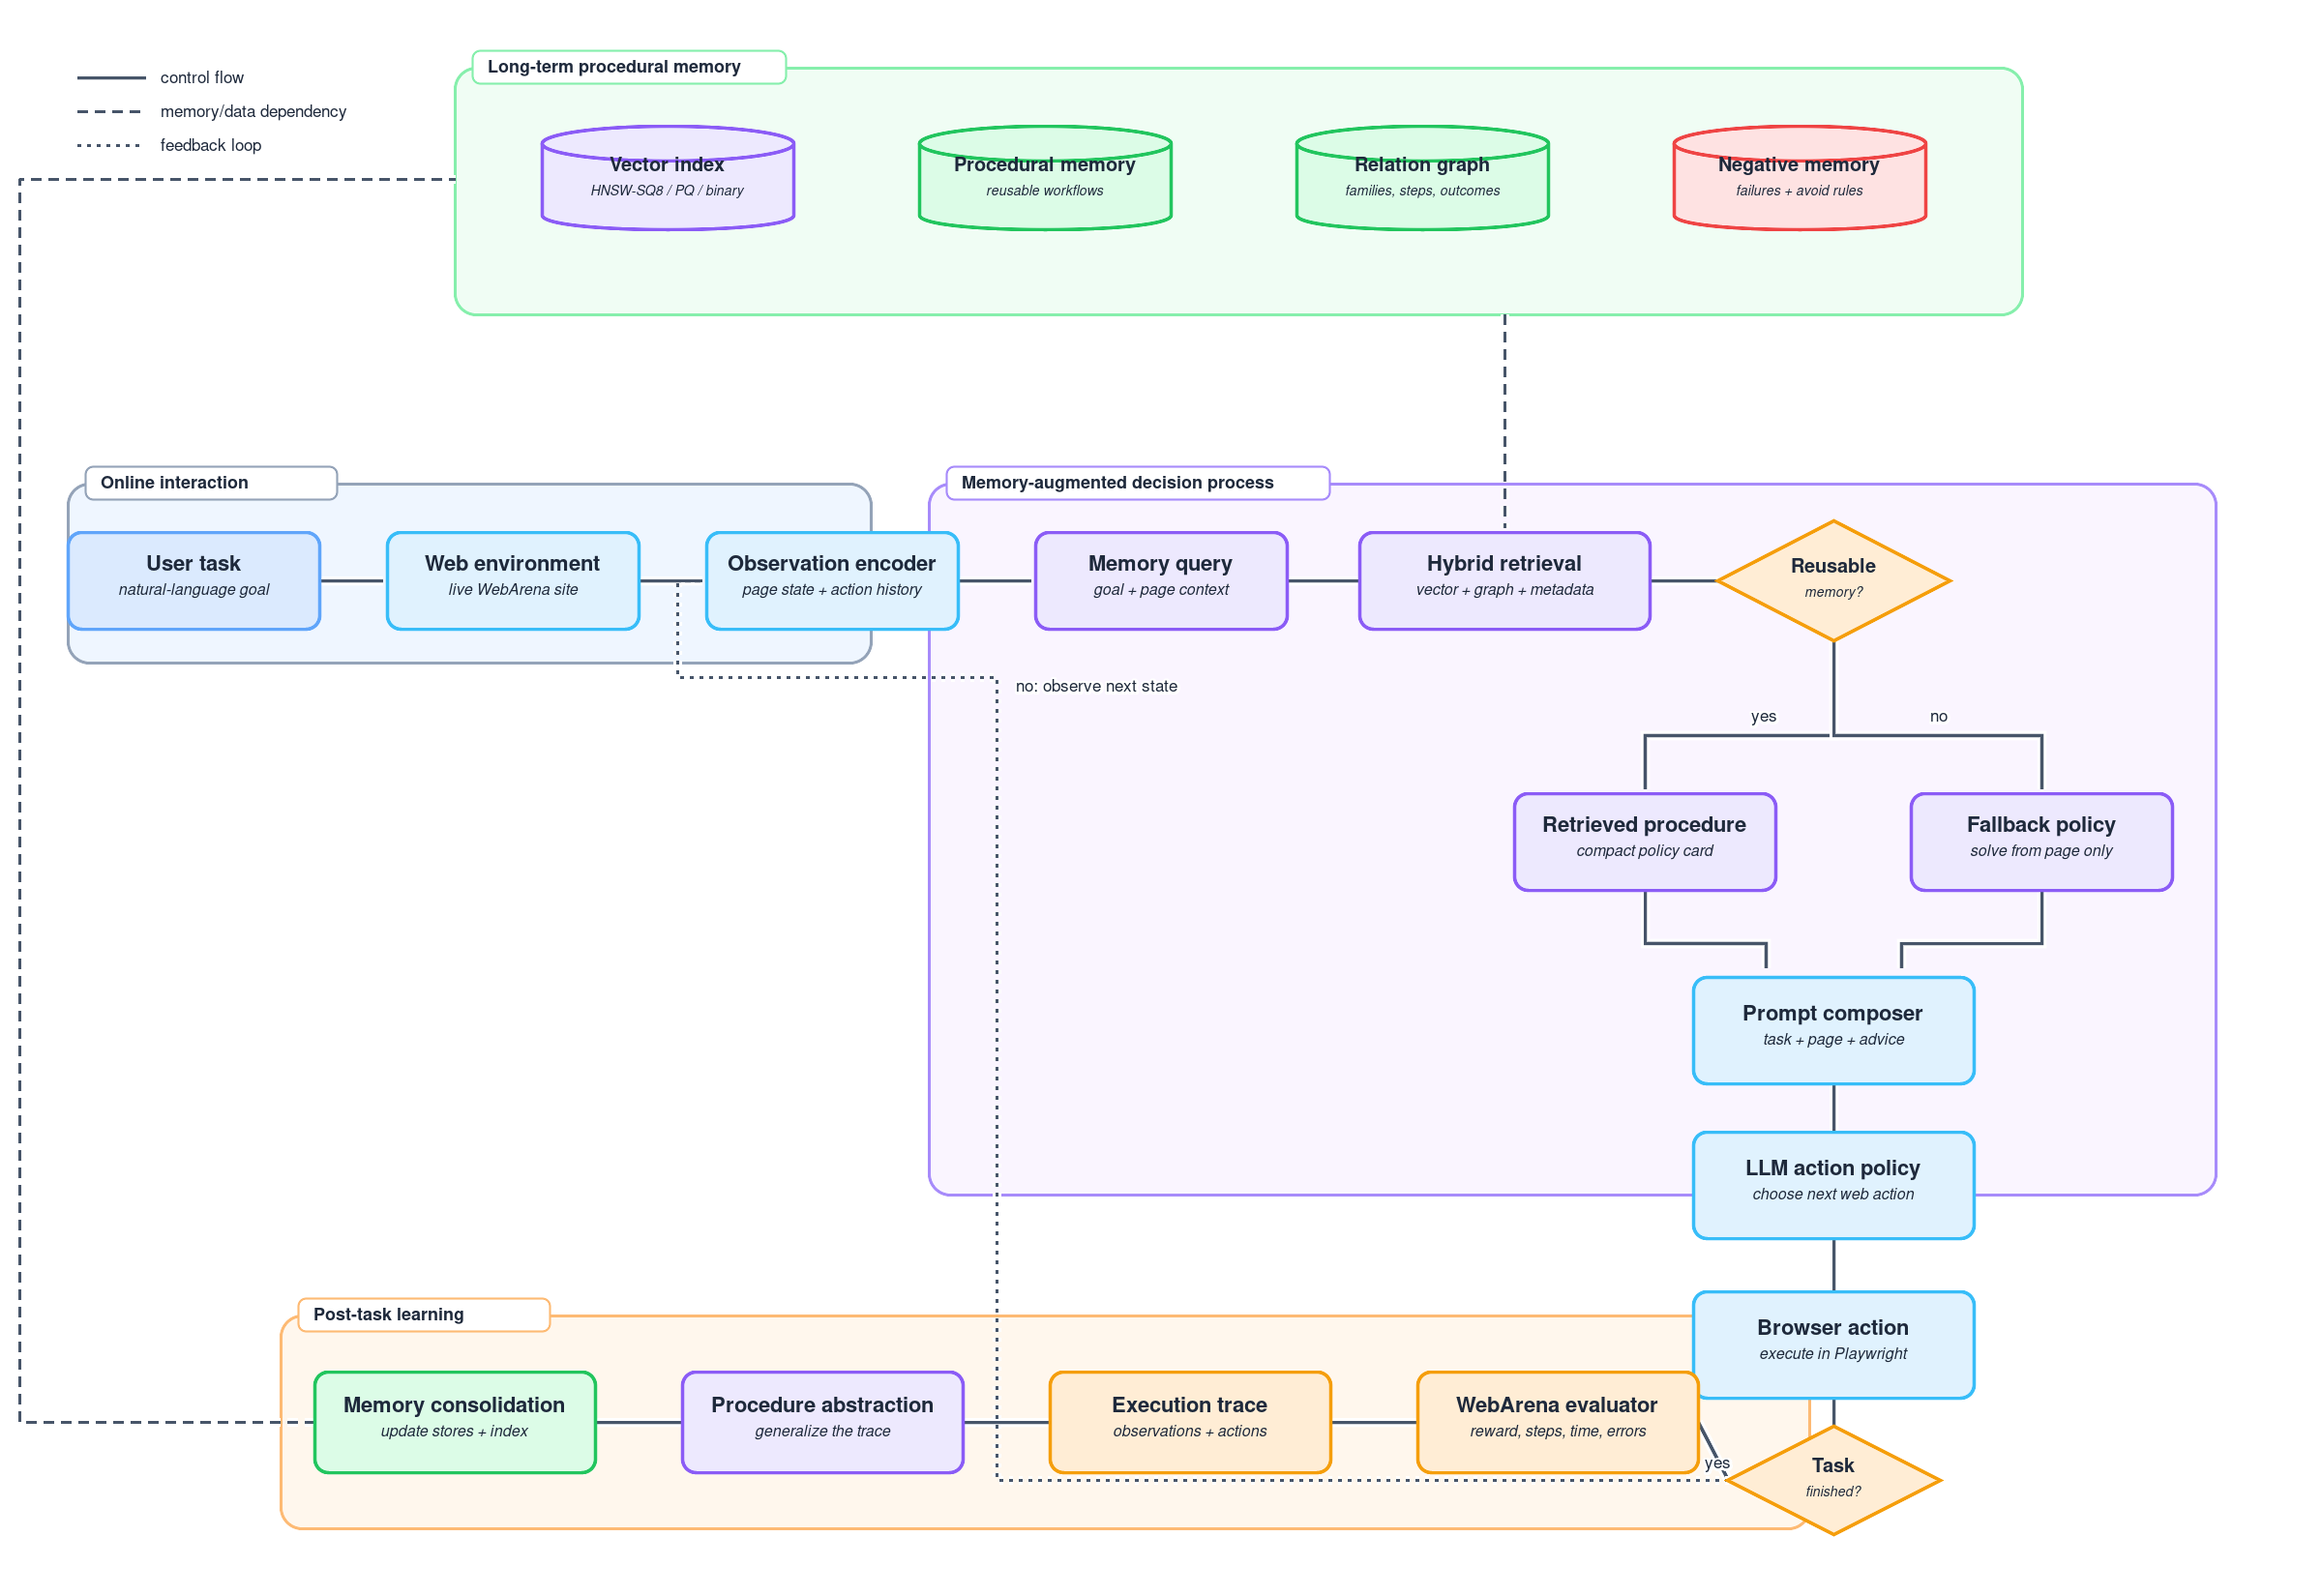
\includegraphics[width=\linewidth]{webarena_procedural_memory_flowchart_paper_clean.png}
  \caption{Paper-level flowchart of the procedural-memory web-agent architecture. A user task is converted into browser observations and a memory query. Hybrid retrieval selects prior procedures or falls back to direct solving. After execution, traces are abstracted into positive or negative procedural memories and update the long-term memory stores.}
  \label{fig:flowchart}
\end{figure}

\subsection{Memory Stores}

The implementation separates long-term memory into several stores:

\begin{table}[h]
\centering
\small
\begin{tabular}{p{0.25\linewidth}p{0.62\linewidth}}
\toprule
\textbf{Store} & \textbf{Purpose} \\
\midrule
Procedural memory & Reusable workflows containing activation conditions, generalized steps, evidence requirements, answer format, and termination conditions. \\
Negative memory & Failure abstractions and avoid-rules, used to penalize memories that resemble previously failed procedures. \\
Relation graph & Edges connecting procedures to task families, sites, action skeletons, UI terms, outcomes, and failure nodes. \\
Vector index & Dense embedding index over compact workflow text. Implemented with FAISS flat, HNSW, SQ8, HNSW+SQ8, IVFPQ, OPQ-IVFPQ, TurboQuant-like binary rotation, and RaBitQ-inspired variants. \\
Relational metadata store & Disk-backed durable tables for procedures, graph edges, negative memories, retrieval events, raw candidates, rejected candidates, and selected candidates. \\
\bottomrule
\end{tabular}
\caption{Major memory stores in the implemented architecture.}
\label{tab:stores}
\end{table}

\subsection{Execution Loop}

In WebArena, the LLM does not directly manipulate the website. BrowserGym and Playwright expose a controlled browser action space. The model receives a text observation produced from the DOM and accessibility tree. Actions such as \texttt{click}, \texttt{fill}, \texttt{scroll}, and \texttt{send\_msg\_to\_user} are executed by Playwright. The EC2 instance hosts the WebArena websites; the external agent runtime calls the LLM through Vertex AI and drives the browser against the hosted services.

\section{Retrieval and Ranking}

\subsection{Embedding Similarity}

Each procedure is rendered into compact text $T(p_i)$ and embedded:
\begin{equation}
  \vect{z}_i = \frac{f_\theta(T(p_i))}{\|f_\theta(T(p_i))\|_2}.
\end{equation}
The query is embedded similarly:
\begin{equation}
  \vect{z}_q = \frac{f_\theta(q)}{\|f_\theta(q)\|_2}.
\end{equation}
Because vectors are L2-normalized, inner product equals cosine similarity:
\begin{equation}
  s_{\mathrm{sem}}(q,p_i)=\vect{z}_q^\top \vect{z}_i.
\end{equation}

\subsection{Hybrid Reranking}

For Mind2Web, the graph-aware procedural reranker combines six signals:
\begin{equation}
\begin{aligned}
  S_{\mathrm{M2W}}(q,p) =
  &0.50s_{\mathrm{sem}} + 0.14s_{\mathrm{lex}} + 0.16s_{\mathrm{act}} \\
  &+0.08s_{\mathrm{graph}} + 0.08s_{\mathrm{out}} + 0.04s_{\mathrm{meta}} - \lambda_{\mathrm{neg}}.
\end{aligned}
\end{equation}
The default acceptance threshold is $0.34$, with an activation floor of $0.04$. The compressed FAISS backend uses a retrieval-first score:
\begin{equation}
  S_{\mathrm{FAISS}}(q,p)=0.78s_{\mathrm{sem}}+0.12s_{\mathrm{lex}}+0.07I_{\mathrm{sameSite}}+0.03I_{\mathrm{sameDomain}}.
\end{equation}
It accepts a memory if either $S_{\mathrm{FAISS}}\ge 0.30$ or $s_{\mathrm{sem}}\ge 0.28$.

For WebArena, the live retriever uses additional task-family and action-structure checks:
\begin{equation}
\begin{aligned}
  S_{\mathrm{WA}}(q,p) =
  &0.42s_{\mathrm{sem}} + 0.16s_{\mathrm{lex}} + 0.18s_{\mathrm{act}}
   +0.06s_{\mathrm{meta}} \\
  &+0.10s_{\mathrm{out}} +0.08s_{\mathrm{graph}}
   +0.22s_{\mathrm{fam}}+0.10s_{\mathrm{struct}} \\
  &-\lambda_{\mathrm{neg}}-\lambda_{\mathrm{mismatch}}.
\end{aligned}
\end{equation}
Same-family candidates require $S_{\mathrm{WA}}\ge0.42$; cross-family candidates require at least $0.48$. If the task family is incompatible, an additional mismatch penalty of $0.22$ is applied.

\subsection{Graph Score}

The relation graph is not a visual graph only; it contributes to ranking. A procedure receives graph score from weighted connectivity to relevant metadata, UI terms, action types, and outcomes. In simplified form:
\begin{equation}
  s_{\mathrm{graph}}(p)=\sigma\left(\sum_{(u,r,p)\in E_q} w_{u,r,p}\right),
\end{equation}
where $E_q$ is the subset of graph edges activated by the current query context and $\sigma$ clips or normalizes the raw edge weight into $[0,1]$. This makes a procedure more reusable when it is strongly connected to the current site, task family, expected UI terms, and successful outcomes.

\section{Procedure Abstraction and Context Compression}

\subsection{Positive Procedural Abstraction}

Raw trajectories are too concrete to reuse directly. They contain transient element ids, long DOM text, and task-specific values. The implemented memory therefore stores an abstract policy card:
\begin{equation}
  p_i = \left(f_i, a_i, k_i, \pi_i, \eta_i, \rho_i\right),
\end{equation}
where $f_i$ is the task family, $a_i$ is the activation condition, $k_i$ is a small keyword/evidence set, $\pi_i$ is the generalized action policy, $\eta_i$ is the expected answer format, and $\rho_i$ is the termination condition. Deterministic abstraction was used in the main Mind2Web retrieval benchmark to isolate memory performance. WebArena later required LLM-based abstraction because live tasks need better semantic generalization and clearer stopping rules.

\subsection{Negative Memory}

For failed tasks, the system stores a negative memory:
\begin{equation}
  n_j = \left(f_j, b_j, \alpha_j, \lambda_j\right),
\end{equation}
where $f_j$ is the failure family, $b_j$ is the bad pattern, $\alpha_j$ is the avoid-rule, and $\lambda_j$ is its penalty. During retrieval, negative memories produce:
\begin{equation}
  \lambda_{\mathrm{neg}}(q,p)=\max_{n_j \in \mathcal{N}} \left[\gamma_f I(f_q=f_j)+\gamma_l s_{\mathrm{lex}}(q,b_j)\right],
\end{equation}
subject to a minimum match gate. This prevents repeated reuse of procedures that look superficially similar but previously failed.

\subsection{Prompt Context Budget}

Instead of placing full trajectories in the prompt, the prompt receives compact policy cards. If a full trace has token length $L_{\tau}$ and its abstract card has length $L_p$, the prompt compression ratio is:
\begin{equation}
  \mathrm{CR}_{\mathrm{prompt}}=\frac{L_{\tau}}{L_p}.
\end{equation}
The online prompt is therefore:
\begin{equation}
  C_t = \left[g, o_t, h_t, \{p_i\}_{i=1}^{k}, \{n_j\}_{j=1}^{m}, r_f\right],
\end{equation}
where $r_f$ are task-family rules. The memory is guidance, not a hard script: the LLM still chooses each action from the current page state.

\section{Storage and Retrieval Optimization}

\subsection{Compression}

A dense embedding of dimension $d=384$ stored as float32 requires:
\begin{equation}
  M_{\mathrm{fp32}} = 4d = 1536 \;\mathrm{bytes/vector}.
\end{equation}
Scalar quantization with 8 bits per dimension stores:
\begin{equation}
  M_{\mathrm{SQ8}} = d = 384 \;\mathrm{bytes/vector}.
\end{equation}
Product quantization with $m=16$ sub-vectors and $b=8$ bits per sub-code stores:
\begin{equation}
  M_{\mathrm{PQ}} = \frac{mb}{8}=16 \;\mathrm{bytes/vector}.
\end{equation}
Thus, for 384-dimensional embeddings, IVFPQ reduces the vector code from 1536 bytes to 16 bytes, a nominal $96\times$ vector-code compression before metadata and index overhead.

Scalar quantization maps each dimension to an 8-bit integer:
\begin{equation}
  Q_{\mathrm{SQ8}}(x_j)=\operatorname{round}\left(255\cdot\frac{x_j-a_j}{b_j-a_j}\right),
\end{equation}
where $a_j$ and $b_j$ are learned or observed bounds for dimension $j$. Product quantization partitions a vector into $m$ subvectors and replaces each subvector with a codebook id:
\begin{equation}
  Q_{\mathrm{PQ}}(\vect{x}) = \left(k_1,\ldots,k_m\right),
  \quad
  k_j=\operatorname*{argmin}_{k}\left\|\vect{x}^{(j)}-\vect{c}_{j,k}\right\|_2^2.
\end{equation}
OPQ first learns a rotation $R$ to reduce quantization error:
\begin{equation}
  R^\star=\operatorname*{argmin}_{R^\top R=I}\sum_i
  \left\|\vect{x}_i - R^\top Q_{\mathrm{PQ}}(R\vect{x}_i)\right\|_2^2.
\end{equation}

\subsection{Index Families}

The implementation evaluates several backends:
\begin{itemize}[leftmargin=*]
  \item \textbf{Flat IP}: exact inner-product search over normalized vectors.
  \item \textbf{HNSW}: graph-based ANN with $M=32$ and efSearch $=64$.
  \item \textbf{SQ8}: scalar-quantized vectors.
  \item \textbf{HNSW+SQ8}: HNSW graph over scalar-quantized vectors.
  \item \textbf{IVFPQ}: inverted-file coarse clustering with product-quantized residual/vector codes.
  \item \textbf{OPQ-IVFPQ}: learned rotation before IVFPQ to reduce quantization error.
  \item \textbf{TurboQuant-like binary rotation}: signed-permutation rotation followed by binary codes.
  \item \textbf{RaBitQ-inspired dense/binary variants}: low-bit randomized quantization experiments.
\end{itemize}

The expected cost of exact search is $O(Nd)$ per query. HNSW reduces the number of visited vectors through greedy graph navigation, empirically close to logarithmic behavior for many high-dimensional collections. IVF reduces search by probing only $n_{\mathrm{probe}}$ coarse clusters:
\begin{equation}
  C_{\mathrm{IVF}}\approx O(n_{\mathrm{probe}}\cdot N/n_{\mathrm{list}}\cdot c_{\mathrm{dist}}),
\end{equation}
where $c_{\mathrm{dist}}$ is the compressed-distance cost. PQ replaces full distance computation with table lookups over sub-codebooks:
\begin{equation}
  \widehat{d}(q,x)=\sum_{j=1}^{m} \left\|q_j - c_{j,k_j(x)}\right\|^2.
\end{equation}

For HNSW, the search state moves greedily through a proximity graph:
\begin{equation}
  v_{t+1}=\operatorname*{argmax}_{u\in \mathcal{N}(v_t)\cup\{v_t\}} \simfn(\vect{z}_q,\vect{z}_u),
\end{equation}
starting from sparse upper layers and refining on denser lower layers. The implementation uses $M=32$ neighbors and efSearch $=64$ in the WebArena HNSW benchmarks.

For binary rotation experiments, a rotated vector is converted to signs:
\begin{equation}
  \vect{b}_i = \operatorname{sign}(R\vect{z}_i),
\end{equation}
and approximate similarity is estimated from agreement or Hamming distance:
\begin{equation}
  \widehat{s}_{\mathrm{bin}}(q,i)=1-\frac{2}{d}H\left(\vect{b}_q,\vect{b}_i\right).
\end{equation}
This gives very small index codes but loses retrieval quality on the small WebArena memory corpus.

\section{Mind2Web Experiments}

\subsection{Evaluation Setup}

The Mind2Web evaluation uses recorded exemplar trajectories with Gemini 2.5 Pro through a Vertex/OpenAI-compatible adapter. The memory policy is same-website procedural reuse. A separate retrieval benchmark isolates the memory subsystem from LLM latency so that retrieval speed, storage cost, and compression behavior can be measured independently. These are local evaluations and should not be represented as an official Mind2Web leaderboard submission.

\subsection{Accuracy Results}

\begin{table}[h]
\centering
\small
\begin{tabular}{lr}
\toprule
\textbf{Metric} & \textbf{Result} \\
\midrule
Element accuracy & 59.76\% \\
Relaxed element accuracy & 95.78\% \\
Operation accuracy & 91.13\% \\
Action F1 & 88.07\% \\
Step success rate & 54.59\% \\
Relaxed step success rate & 84.67\% \\
Task success rate & 11.60\% \\
Relaxed task success rate & 45.00\% \\
Exact sequence rate & 11.00\% \\
\bottomrule
\end{tabular}
\caption{Mind2Web procedural evaluation results.}
\label{tab:mind2web_accuracy}
\end{table}

\begin{table}[h]
\centering
\small
\begin{tabular}{lrrr}
\toprule
\textbf{Metric} & \textbf{This method} & \textbf{AWM reference} & \textbf{Delta} \\
\midrule
Element accuracy & 59.76\% & 50.60\% & +9.16 pts \\
Action F1 & 88.07\% & 57.30\% & +30.77 pts \\
Step success rate & 54.59\% & 45.10\% & +9.49 pts \\
Task success rate & 11.60\% & 4.80\% & +6.80 pts \\
\bottomrule
\end{tabular}
\caption{Comparison against the strongest AWM Mind2Web reference values used in this study. The comparison is useful for orientation but is not an official reproduction because the local evaluation setup, model, and data protocol differ from the original paper.}
\label{tab:mind2web_paper_comparison}
\end{table}

\subsection{Retrieval Benchmark}

\begin{table}[h]
\centering
\small
\begin{tabular}{lrrrrrr}
\toprule
\textbf{Backend} & \textbf{Acceptance} & \textbf{Total s} & \textbf{Avg ms} & \textbf{P95 ms} & \textbf{RSS +MB} & \textbf{Code bytes} \\
\midrule
RAM FAISS+BM25 & 99.0\% & 72.57 & 40.50 & 64.29 & 167.31 & -- \\
Compressed FAISS IVFPQ & 99.8\% & 39.68 & 26.16 & 38.65 & 155.51 & 16 \\
\bottomrule
\end{tabular}
\caption{Mind2Web memory-backend benchmark. The compressed backend removes Python vector storage and uses 16-byte FAISS PQ codes.}
\label{tab:mind2web_retrieval}
\end{table}

The benchmark demonstrates that the memory layer can be made significantly more efficient without reducing retrieval acceptance. Relative to the RAM FAISS baseline, compressed FAISS reduces average retrieval latency by 35.4\%, reduces P95 latency by 39.9\%, lowers total benchmark runtime by 45.3\%, and slightly increases the accepted-retrieval rate.

\section{WebArena Experiments}

\subsection{Live Browser Setup}

The WebArena stack is hosted on an EC2 instance. The agent runtime, BrowserGym, Playwright, procedural memory, and LLM adapter run externally and interact with the hosted websites through browser automation. The key distinction from Mind2Web is that WebArena is live: tasks can fail because of navigation timing, browser loops, page loading, answer formatting, or environment availability. Therefore, WebArena evaluates both the reasoning policy and the reliability of the execution system.

\subsection{Live Shopping-Domain Results}

\begin{table}[h]
\centering
\small
\begin{tabular}{lr}
\toprule
\textbf{Metric} & \textbf{Value} \\
\midrule
Success rate & 58.62\% \\
Average steps/task & 3.41 \\
Procedures in memory & 19 \\
Procedure edges & 256 \\
Negative memories & 28 \\
Retrieval events & 380 \\
Selected retrieval events & 306 \\
Overall selected rate & 80.5\% \\
Memory storage & $\approx$3.2 MB \\
\bottomrule
\end{tabular}
\caption{WebArena shopping-domain procedural-memory evaluation.}
\label{tab:webarena_best}
\end{table}

\subsection{WebArena Retrieval Backend Benchmark}

\begin{table}[h]
\centering
\scriptsize
\begin{tabular}{lrrrrr}
\toprule
\textbf{Backend} & \textbf{Actual index} & \textbf{Avg ms} & \textbf{P95 ms} & \textbf{Top-k match} & \textbf{Index bytes} \\
\midrule
Flat & flat IP & 21.59 & 25.66 & 82.8\% & 33,837 \\
HNSW & HNSW $M=32$ & 20.55 & 23.09 & 82.8\% & 39,914 \\
SQ8 & scalar quantized & 21.53 & 30.08 & 85.6\% & 11,601 \\
HNSW+SQ8 & HNSW over SQ8 & 21.78 & 29.02 & 85.6\% & 17,678 \\
IVFPQ & fallback to HNSW+SQ8 & 25.12 & 36.27 & 85.6\% & 17,678 \\
OPQ-IVFPQ & fallback to HNSW+SQ8 & 23.99 & 29.92 & 85.6\% & 17,678 \\
TurboQuant-like & signed permutation binary & 21.59 & 27.64 & 72.8\% & 1,089 \\
RaBitQ-inspired & dense binary & 121.73 & 139.82 & 58.0\% & 1,089 \\
Binary HNSW rotation & binary HNSW & 24.06 & 32.61 & 72.8\% & 7,154 \\
\bottomrule
\end{tabular}
\caption{WebArena retrieval-backend benchmark using a small shopping-domain memory corpus with BAAI/bge-small-en-v1.5 embeddings. IVFPQ and OPQ-IVFPQ fall back because the corpus is below the PQ training requirement.}
\label{tab:webarena_backend}
\end{table}

In the small-memory setting, embedding and runtime overhead dominate; all non-degenerate dense indexes cluster around 20--25 ms. The more important result is the space--recall frontier: SQ8 and HNSW+SQ8 preserve the best top-k reference match rate (85.6\%) while reducing index bytes relative to flat search; binary methods are far smaller but lose retrieval quality in this setting.

\section{Qualitative Findings}

\paragraph{Mind2Web.}
The strongest Mind2Web result is that compact procedural memory can improve full-task success while keeping retrieval fast. The main remaining weakness is exact element grounding. Relaxed element accuracy is high (95.78\%), operation accuracy is high (91.13\%), and action F1 is high (88.07\%), but strict element accuracy remains lower. This suggests that the model usually understands the action intent but sometimes selects a neighboring, nested, or equivalent element that fails strict matching.

\paragraph{WebArena.}
WebArena failures were more operationally diverse. Observed failure modes include:
\begin{itemize}[leftmargin=*]
  \item no memory retrieved because task families were too different or thresholds were too strict;
  \item looping on sort/pagination controls even after enough evidence was available;
  \item evaluator-sensitive answer formatting;
  \item navigation timing errors such as execution-context destruction while pages were loading;
  \item weak early abstraction before mandatory LLM-based abstraction was added;
  \item EC2 availability or proxy failures during live experiments.
\end{itemize}
Fixes included LLM-based positive and negative abstraction, stricter stop conditions, loop detection for price-range tasks, more retries, wait-after-action improvements, task-family guardrails, and logging of selected, rejected, and raw retrieval candidates.

\section{Discussion}

The central lesson is that memory quality and memory systems design are inseparable. A web-agent memory can fail in at least three ways: it can store overly concrete traces, retrieve irrelevant traces, or inject too much context into the prompt. The proposed architecture addresses these failure modes by separating full evidence from compact retrieval text, storing negative memory, requiring thresholded retrieval, and composing only compact policy cards into the prompt.

For small memories, the LLM dominates runtime. However, at large scale the retrieval system becomes a first-class bottleneck. A billion workflows with 384-dimensional float32 embeddings would require approximately:
\begin{equation}
  10^9 \times 1536 \;\mathrm{bytes} \approx 1.536\;\mathrm{TB}
\end{equation}
for raw vector values alone, before metadata and graph edges. With 16-byte PQ codes, the vector-code portion becomes:
\begin{equation}
  10^9 \times 16 \;\mathrm{bytes} = 16\;\mathrm{GB}.
\end{equation}
This motivates IVFPQ, OPQ, DiskANN-style disk-resident indexes, binary quantization, and learned reranking for future large-scale procedural memory.

\section{Limitations}

This project is a strong implementation study but has limitations:
\begin{itemize}[leftmargin=*]
  \item The Mind2Web comparison is based on a local evaluation, not an official paper reproduction.
  \item The WebArena results focus on the shopping domain.
  \item WebArena memory is still small, so billion-scale ANN backends cannot be fully validated from these data alone.
  \item Binary/TurboQuant/RaBitQ-style variants are experimental approximations, not full paper-faithful implementations.
  \item LLM-based abstraction quality can vary, and malformed abstraction responses can cause skipped memory ingestion unless recovery logic is used.
  \item Live browser experiments depend on EC2 uptime, proxy behavior, page timing, and evaluator formatting.
\end{itemize}

\section{Future Work}

The next stage should evaluate multi-domain WebArena tasks, increase the memory corpus size, and measure retrieval under larger synthetic and real workflow collections. The most important engineering directions are:
\begin{enumerate}[leftmargin=*]
  \item \textbf{Disk-resident ANN:} integrate DiskANN-style indexes for memory corpora that do not fit in RAM.
  \item \textbf{Learned reranking:} replace fixed feature weights with a trained reranker over successful and failed retrieval events.
  \item \textbf{Hierarchical memory:} retrieve first by task family, then workflow, then step-level action policy.
  \item \textbf{Adaptive thresholds:} tune memory acceptance thresholds from historical success/failure outcomes.
  \item \textbf{Better embeddings:} compare BGE-small, BGE-base/large, E5, and task-specific workflow encoders under equal latency budgets.
  \item \textbf{Multimodal observations:} add screenshot-capable policies for visual tasks where DOM/accessibility text is insufficient.
  \item \textbf{Production telemetry:} track retrieval latency, prompt tokens, selected memory ids, step count, loop breaks, final reward, and memory growth per evaluation.
\end{enumerate}

\section{Conclusion}

This project implements a practical procedural-memory system for web agents across Mind2Web and WebArena. The Mind2Web results show that workflow memory with Gemini 2.5 Pro can outperform tracked AWM paper references under the local evaluation setup, while compressed FAISS IVFPQ substantially improves retrieval latency and storage efficiency. The WebArena results show that live browser agents require more than vector search: they need graph-guided memory, negative memories, LLM-based abstraction, action-loop guards, robust browser waits, and careful answer formatting. Overall, the work supports a production-oriented view of web-agent memory: reusable procedures should be abstracted, indexed, compressed, graph-linked, logged, and selectively injected into the agent prompt.

\appendix

\section{Evaluation Protocol Details}

All reported metrics are computed from saved experimental outputs produced during the project. Mind2Web metrics are step-level and task-level offline evaluation metrics over recorded exemplar trajectories. WebArena metrics are live-environment task outcomes over a shopping-domain subset, where success is determined by the WebArena evaluator. Retrieval benchmarks are measured separately from live browser execution to isolate the memory subsystem from LLM latency and website timing effects.

\begin{thebibliography}{99}

\bibitem{wang2024awm}
Zora Zhiruo Wang, Jiayuan Mao, Daniel Fried, and Graham Neubig.
\newblock Agent Workflow Memory.
\newblock \emph{arXiv preprint arXiv:2409.07429}, 2024.

\bibitem{deng2023mind2web}
Xiang Deng, Yu Gu, Boyuan Zheng, Shijie Chen, Samuel Stevens, Boshi Wang, Huan Sun, and Yu Su.
\newblock Mind2Web: Towards a Generalist Agent for the Web.
\newblock \emph{arXiv preprint arXiv:2306.06070}, 2023.

\bibitem{zhou2023webarena}
Shuyan Zhou, Frank F. Xu, Hao Zhu, Xuhui Zhou, Robert Lo, Abishek Sridhar, Xianyi Cheng, Tianyue Ou, Yonatan Bisk, Daniel Fried, Uri Alon, and Graham Neubig.
\newblock WebArena: A Realistic Web Environment for Building Autonomous Agents.
\newblock \emph{arXiv preprint arXiv:2307.13854}, 2023.

\bibitem{dechezelles2024browsergym}
Thibault Le Sellier De Chezelles, Maxime Gasse, Alexandre Drouin, Massimo Caccia, Leo Boisvert, Megh Thakkar, Tom Marty, Rim Assouel Shayegan, Lawrence Keunho Jang, Xing Han Lu, Ori Yoran, Dehan Kong, Frank F. Xu, Siva Reddy, Quentin Cappart, Graham Neubig, Ruslan Salakhutdinov, Nicolas Chapados, and Alexandre Lacoste.
\newblock The BrowserGym Ecosystem for Web Agent Research.
\newblock \emph{arXiv preprint arXiv:2412.05467}, 2024.

\bibitem{johnson2017faiss}
Jeff Johnson, Matthijs Douze, and Herv\'e J\'egou.
\newblock Billion-scale similarity search with GPUs.
\newblock In \emph{Proceedings of the IEEE International Conference on Big Data}, 2017.

\bibitem{malkov2020hnsw}
Yu. A. Malkov and D. A. Yashunin.
\newblock Efficient and robust approximate nearest neighbor search using Hierarchical Navigable Small World graphs.
\newblock \emph{IEEE Transactions on Pattern Analysis and Machine Intelligence}, 42(4):824--836, 2020.

\bibitem{jegou2011pq}
Herv\'e J\'egou, Matthijs Douze, and Cordelia Schmid.
\newblock Product Quantization for Nearest Neighbor Search.
\newblock \emph{IEEE Transactions on Pattern Analysis and Machine Intelligence}, 33(1):117--128, 2011.

\bibitem{ge2013opq}
Tiezheng Ge, Kaiming He, Qifa Ke, and Jian Sun.
\newblock Optimized Product Quantization for Approximate Nearest Neighbor Search.
\newblock In \emph{Proceedings of the IEEE Conference on Computer Vision and Pattern Recognition}, pages 2946--2953, 2013.

\bibitem{subramanya2019diskann}
Suhas Jayaram Subramanya, Fnu Devvrit, Harsha Vardhan Simhadri, Ravishankar Krishnaswamy, and Rohan Kadekodi.
\newblock DiskANN: Fast Accurate Billion-point Nearest Neighbor Search on a Single Node.
\newblock In \emph{Advances in Neural Information Processing Systems}, 2019.

\bibitem{guo2019avq}
Ruiqi Guo, Philip Sun, Erik Lindgren, Quan Geng, David Simcha, Felix Chern, and Sanjiv Kumar.
\newblock Accelerating Large-Scale Inference with Anisotropic Vector Quantization.
\newblock \emph{arXiv preprint arXiv:1908.10396}, 2019.

\bibitem{reimers2019sentencebert}
Nils Reimers and Iryna Gurevych.
\newblock Sentence-BERT: Sentence Embeddings using Siamese BERT-Networks.
\newblock In \emph{Proceedings of the 2019 Conference on Empirical Methods in Natural Language Processing}, pages 3982--3992, 2019.

\bibitem{chen2024bge}
Jianlv Chen, Shitao Xiao, Peitian Zhang, Kun Luo, Defu Lian, and Zheng Liu.
\newblock BGE M3-Embedding: Multi-Lingual, Multi-Functionality, Multi-Granularity Text Embeddings Through Self-Knowledge Distillation.
\newblock \emph{arXiv preprint arXiv:2402.03216}, 2024.

\bibitem{gao2024rabitq}
Jianyang Gao and Cheng Long.
\newblock RaBitQ: Quantizing High-Dimensional Vectors with a Theoretical Error Bound for Approximate Nearest Neighbor Search.
\newblock \emph{arXiv preprint arXiv:2405.12497}, 2024.

\bibitem{zandieh2025turboquant}
Amir Zandieh, Majid Daliri, Majid Hadian, and Vahab Mirrokni.
\newblock TurboQuant: Online Vector Quantization with Near-optimal Distortion Rate.
\newblock \emph{arXiv preprint arXiv:2504.19874}, 2025.

\bibitem{yao2023react}
Shunyu Yao, Jeffrey Zhao, Dian Yu, Nan Du, Izhak Shafran, Karthik Narasimhan, and Yuan Cao.
\newblock ReAct: Synergizing Reasoning and Acting in Language Models.
\newblock In \emph{International Conference on Learning Representations}, 2023.

\end{thebibliography}

\end{document}
